\chapter{Discussion}



\section{Application}

\subsection{Home application}
The beamforming array might be quite big for home application, but it may be possible to reduce the size of the beamforming array with smaller speaker units. At this point there are several possibility for home application. Imagen that the house is designed and built as an open living environment, where the kitchen and the living room is a combined open area. There might be a television with stereo speakers in the living room where the back for the television and the back of speaker points towards the kitchen. The low frequency might be an issue backwards because a low frequency driver radiate omnidirectional. At higher frequency the power is more radiated agents the person that watch television, because the high frequency driver is cardioid in it self, only the reflection reflect back to the kitchen. Because of this directionality, there might be higher pressure in the kitchen of the low frequency than the high frequency. Therefore the sound might be annoying in the kitchen because it is dominated by the low frequency. A simulation of a indoor situation with 2 speaker array is a living room is done in \autoref{fig:Indoor_simulation_60_100} and \autoref{fig:Indoor_simulation_200_300}
 




\subsection{Monitor}
Using a normal monitor for monitor application might have some complications, where the monitor and the microphone make a feedback loop or the performer is ignored by the neighbour performer monitor. The beamforming array cannot solve the feedback loop, but the beamforming array will lower the pressure in side of the monitor at low frequency and might have an useful effect. This application both have a posential at stage inside and outside. The problem of using this inside can be that the reflection is so strong that the effect do not work as intended. Another problem with monitor might be that the stage is small and there is barely space for the monitor. By adding additional input and filter for different direction of the beamforming array, it might be possible to take away three monitors and replace them by one beamforming array on such small stage. By narrow the front beam and allow higher beam at the back the sound might be possible to point on the performer as wanted. This kind of bemforming require further investigation and designing which not is done in this project. A simulation is made of a indoor application where two monitors of the beemforming array are placed on a stage, see \autoref{sec:dis:simulation}



\subsection{Main application}
The main application of the beamforming array was intended to outdoor venue, where the neighbour was the non voluntary listener. In this application where the speaker is under free field condition, it have been shown that the sound pressure can be attenuated at least \SI{-9}{\decibel} at the back and side of the array. Therefore the beamforming array will help damping the this kind of side effect of outdoor concert.


\subsection{Simulation}\label{sec:dis:simulation}
The aim of this section is to shortly investigate the wave behaver of the speaker array inside with wall reflection. This project have covered the design of the beamforming array and the behaver in free field condition. The indoor application have been keep out of interest, because of the starting point of application, which have been focused on outdoor event. The last point in the introduction was questioning the indoor application of the beamforming array. At this point there is many possibility since every room is different. The room could be a big concert hall or just a small room for living. It have been chosen to simulate a concert hall because of the monitoring application and the living room for home application. For the living room, it have been chosen to use a standard listening room of size (\SI{4.15}{\meter} x \SI{7.8}{\meter}) which correspond to the \gls{aau} standard listening room. All simulation will be done in 2 dimension because of the computation time and memory requirement. It will not give the exact simulation of the room, but since the reflection coefficient of the room wall not is measured there is already many unknown parameters in this simulation. Therefore the simulation give an impression of the wave behaviour in the room and not valid result. The result from a simulation of a size like the listening room is shown in \autoref{fig:Indoor_simulation_60_100} and \autoref{fig:Indoor_simulation_200_300}



\begin{figure}[H]
\begin{subfigure}[c]{0.5\textwidth}
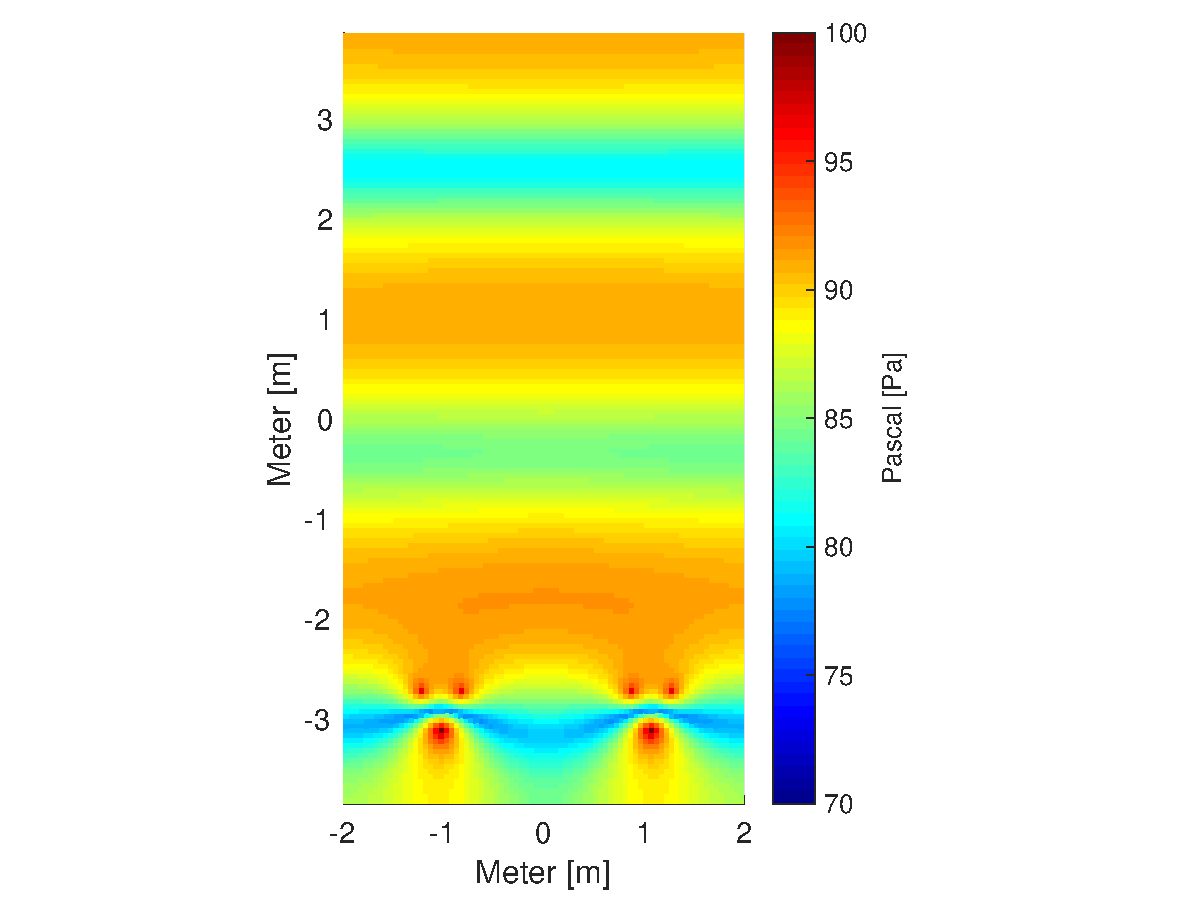
\includegraphics[width=0.95\textwidth]{60_hz_inside_beam.eps}
\subcaption{Indoor simulation of  \SI{60}{\hertz} with beamforming}
\label{fig:Indoor_simulation_60_on}
\end{subfigure}
\begin{subfigure}[c]{0.5\textwidth}
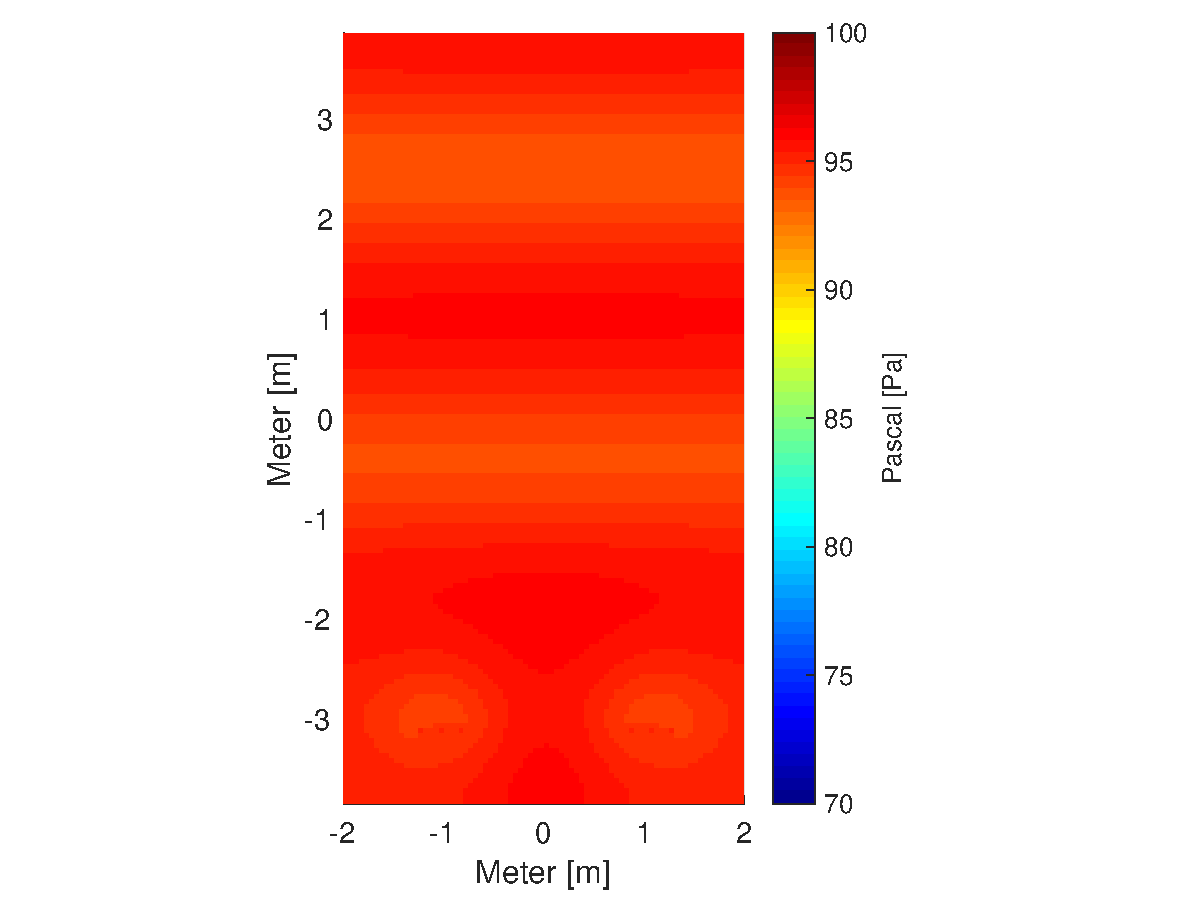
\includegraphics[width=0.95\textwidth]{60_hz_inside_without_beam.eps}
\subcaption{Indoor simulation of  \SI{60}{\hertz} without beamforming}
\label{fig:Indoor_simulation_60_off}
\end{subfigure}\\
\hspace{0.1\textheight}
\begin{subfigure}[c]{0.5\textwidth}
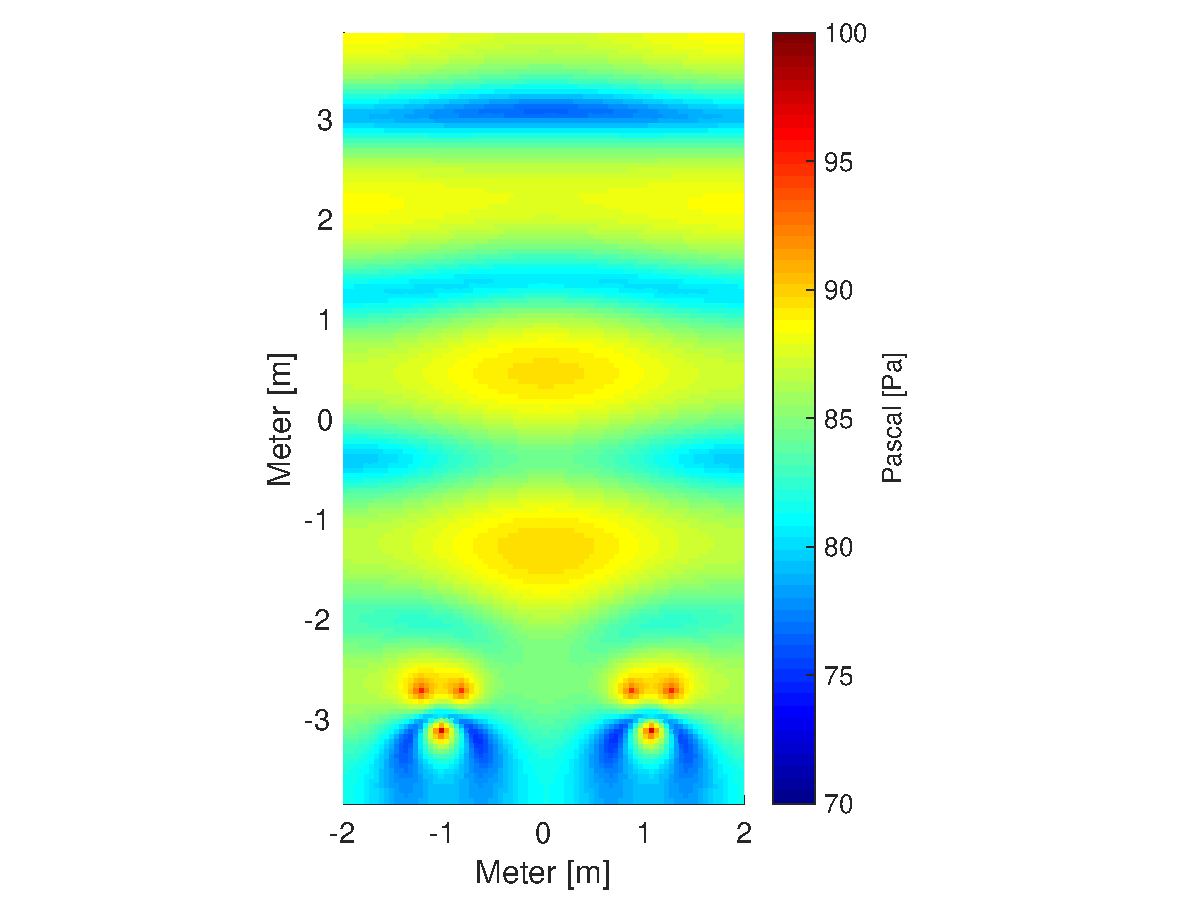
\includegraphics[width=0.95\textwidth]{100_hz_inside_beam.eps}
\subcaption{Indoor simulation of  \SI{100}{\hertz} with beamforming}
\label{fig:Indoor_simulation_100_on}
\end{subfigure}
\begin{subfigure}[c]{0.5\textwidth}
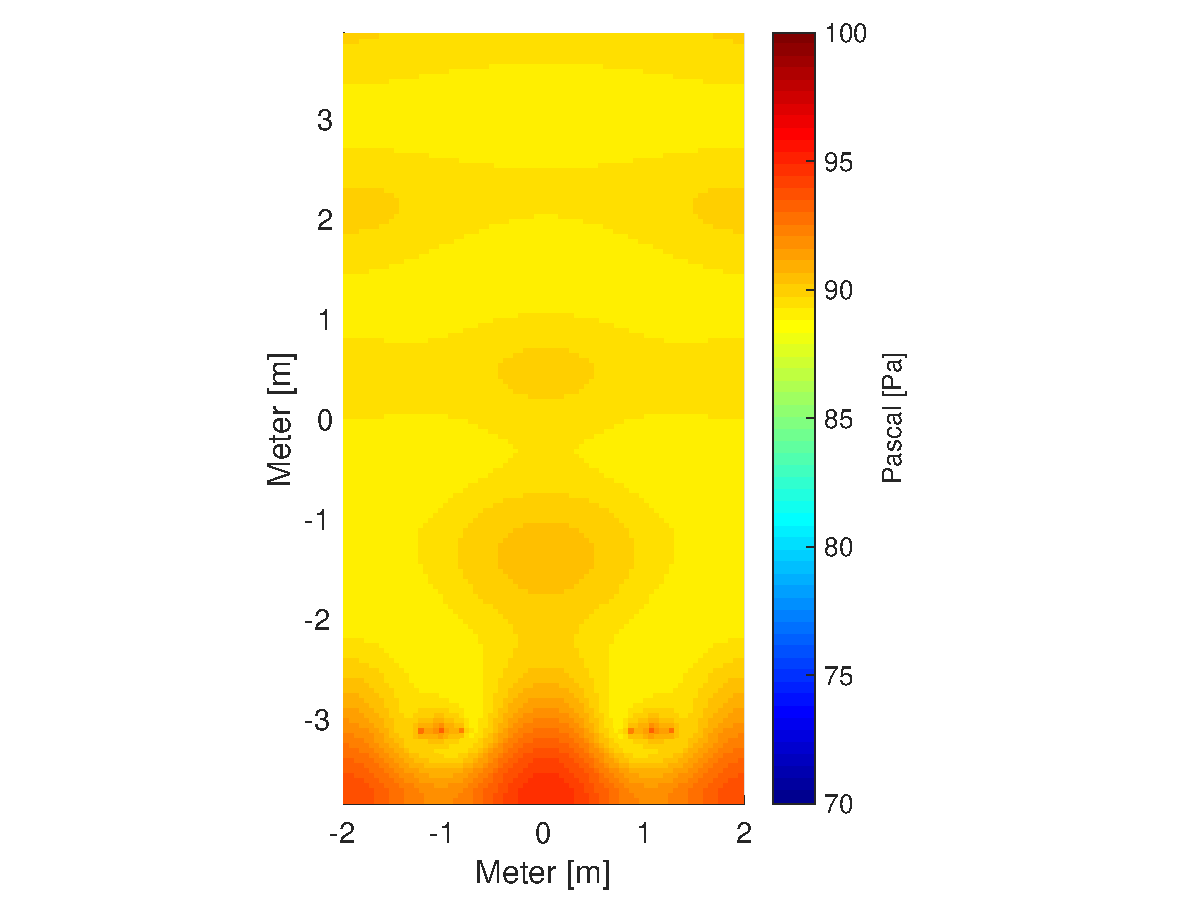
\includegraphics[width=0.95\textwidth]{100_hz_inside_without_beam.eps}
\subcaption{Indoor simulation of  \SI{100}{\hertz} with beamforming}
\label{fig:Indoor_simulation_100_off}
\end{subfigure}
\caption{The figure shows a 2 dimension \gls{fdtd} simulation in a room of size  (\SI{4.15}{\meter} x \SI{7.8}{\meter})}
		\label{fig:Indoor_simulation_60_100}
\end{figure}


\begin{figure}[H]
\begin{subfigure}[c]{0.5\textwidth}
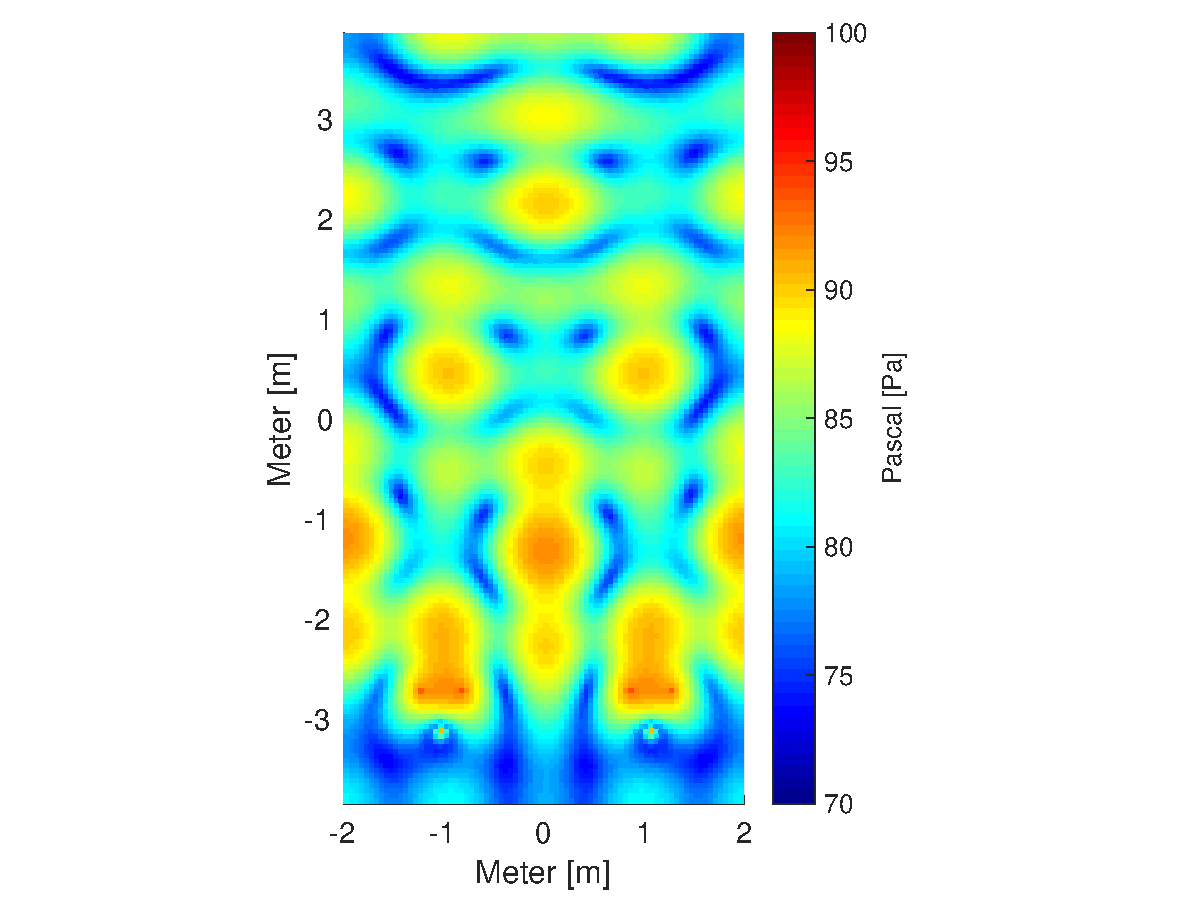
\includegraphics[width=0.95\textwidth]{200_hz_inside_beam.eps}
\subcaption{Indoor simulation of  \SI{200}{\hertz} with beamforming}
\label{fig:Indoor_simulation_200_on}
\end{subfigure}
\begin{subfigure}[c]{0.5\textwidth}
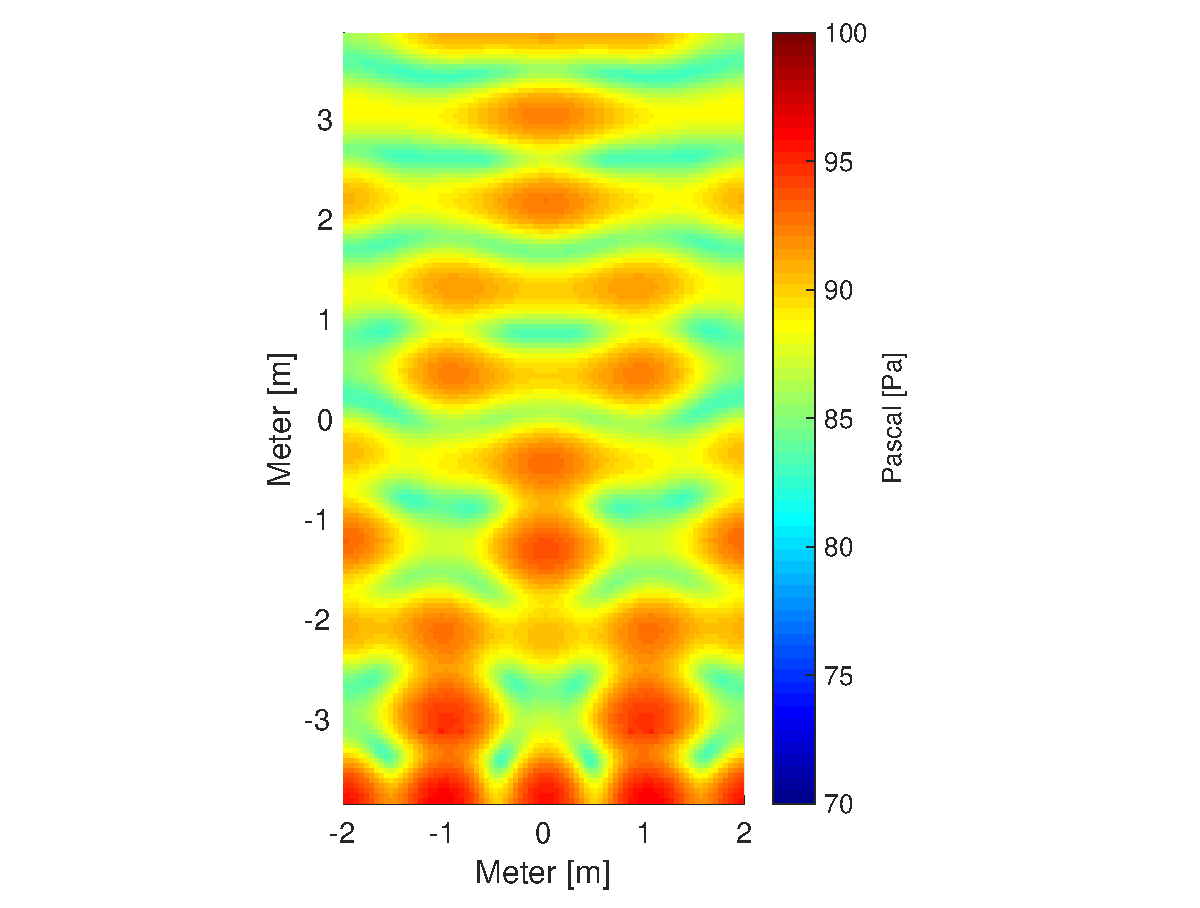
\includegraphics[width=0.95\textwidth]{200_hz_inside_without_beam.eps}
\subcaption{Indoor simulation of  \SI{200}{\hertz} without beamforming}
\label{fig:Indoor_simulation_200_off}
\end{subfigure}
\begin{subfigure}[c]{0.5\textwidth}
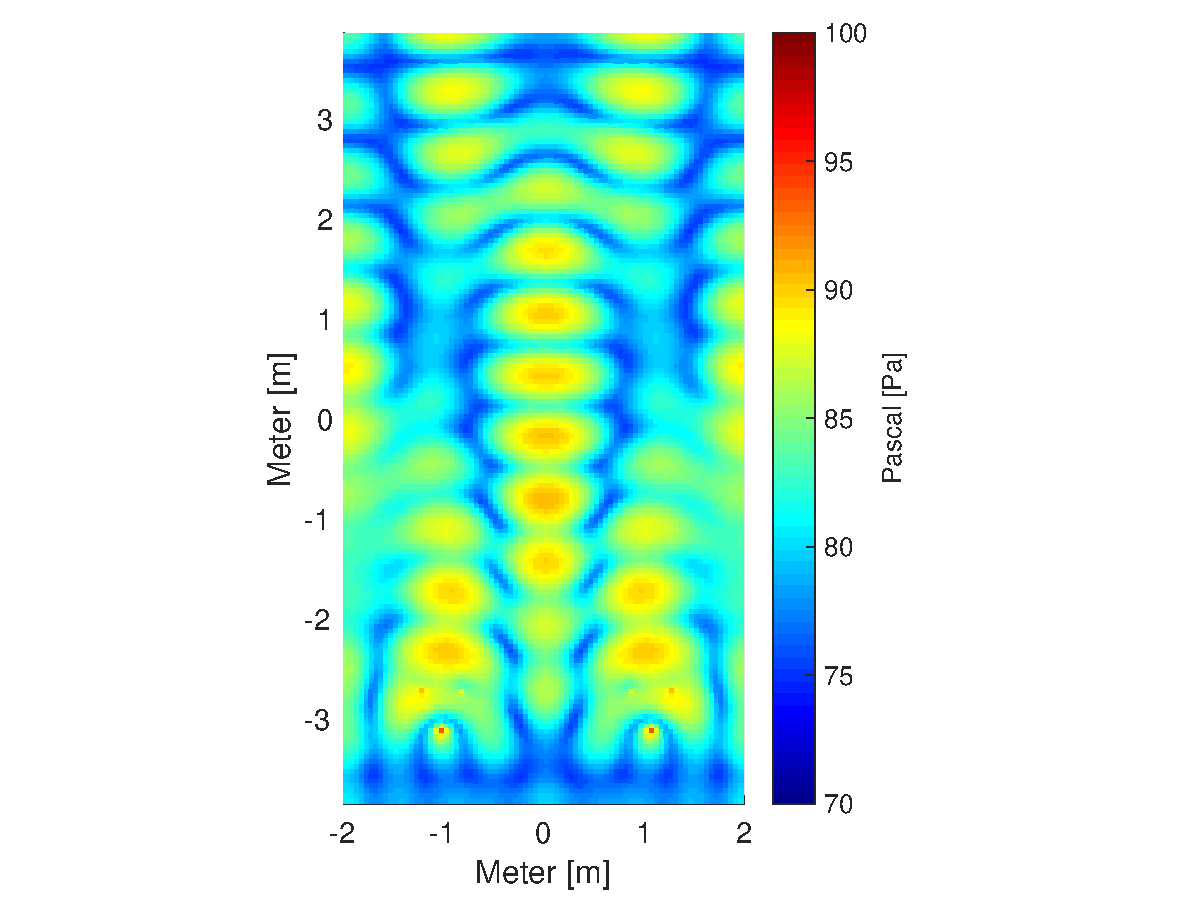
\includegraphics[width=0.95\textwidth]{300_hz_inside_beam.eps}
\subcaption{Indoor simulation of  \SI{300}{\hertz} with beamforming}
\label{fig:Indoor_simulation_300_on}
\end{subfigure}
\begin{subfigure}[c]{0.5\textwidth}
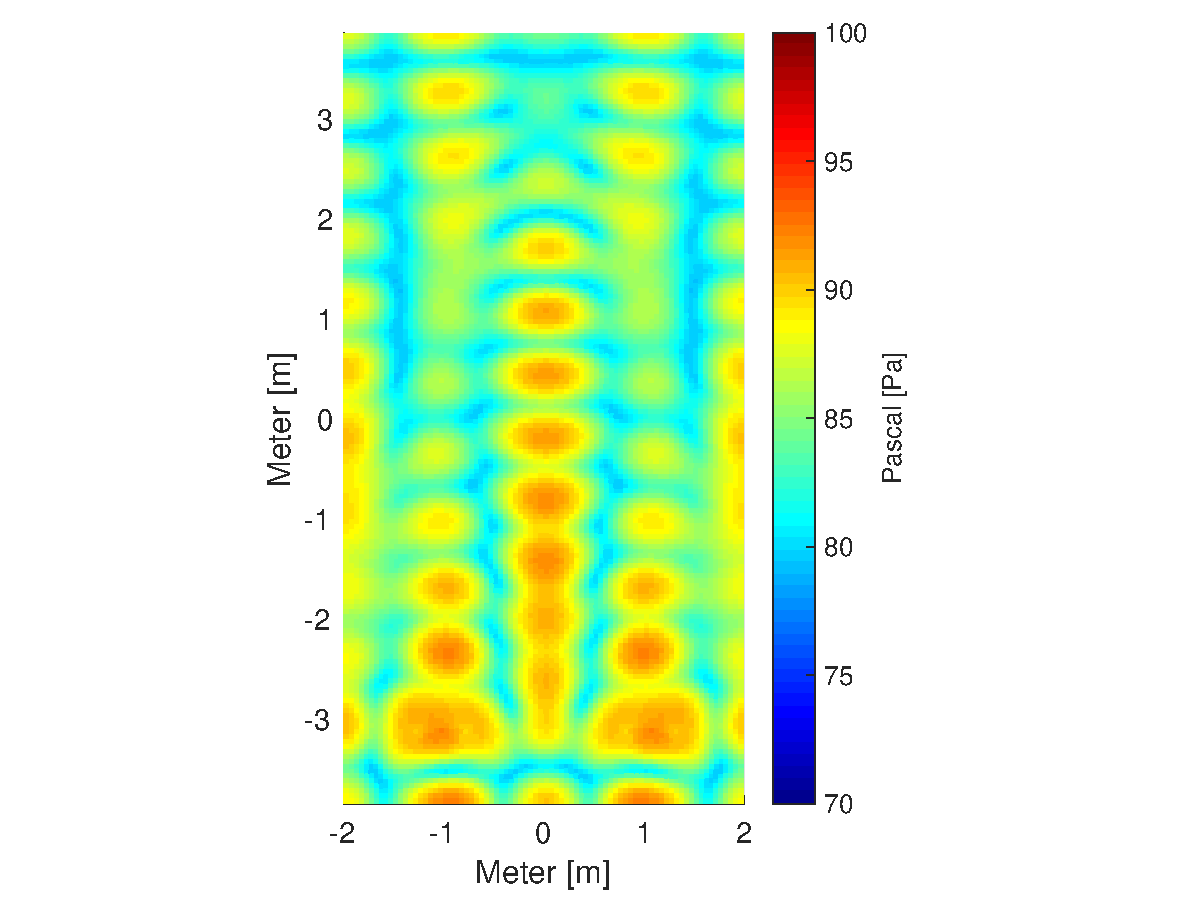
\includegraphics[width=0.95\textwidth]{300_hz_inside_without_beam.eps}
\subcaption{Indoor simulation of  \SI{300}{\hertz} without beamforming}
\label{fig:Indoor_simulation_300_off}
\end{subfigure}
\caption{The figure shows a 2 dimension \gls{fdtd} simulation in a room of size  (\SI{4.15}{\meter} x \SI{7.8}{\meter})}
		\label{fig:Indoor_simulation_200_300}
\end{figure}

In \autoref{fig:Indoor_simulation_60_100} and \autoref{fig:Indoor_simulation_200_300} it can be seen that the pressure in the room is not even ether with beamforming active or not. But one notable thing is that the pressure in the room at low frequency with omnidirectional array gets very high compare to higher frequency. So the room amplify the low frequency with reflection more that in the higher frequency area. The pressure seems to be more frequency pressure constant with beamforming active compare to beamforming disabled.\\


A second indoor application is the monitoring. In a monitoring application the room tens to be larger than a living room. The use of monitoring is often to both small and big concert where both dedicated concert hall and sports arenas are used. The following simulating example are done in a sports arena where the spectator area are on the long side of the playing field. An handball playing field do have a size of (\SI{20}{\meter}x\SI{40}{\meter}) and in this case the spectator is \SI{5}{\meter} on both long side. The following simulation \autoref{fig:Indoor_monitor_60_300} shows a simulation where the stage is placed on the top of the simulation with two monitor. Both monitors is playing upwards when looking at the simulation.


\begin{figure}[H]
\begin{subfigure}[c]{0.5\textwidth}
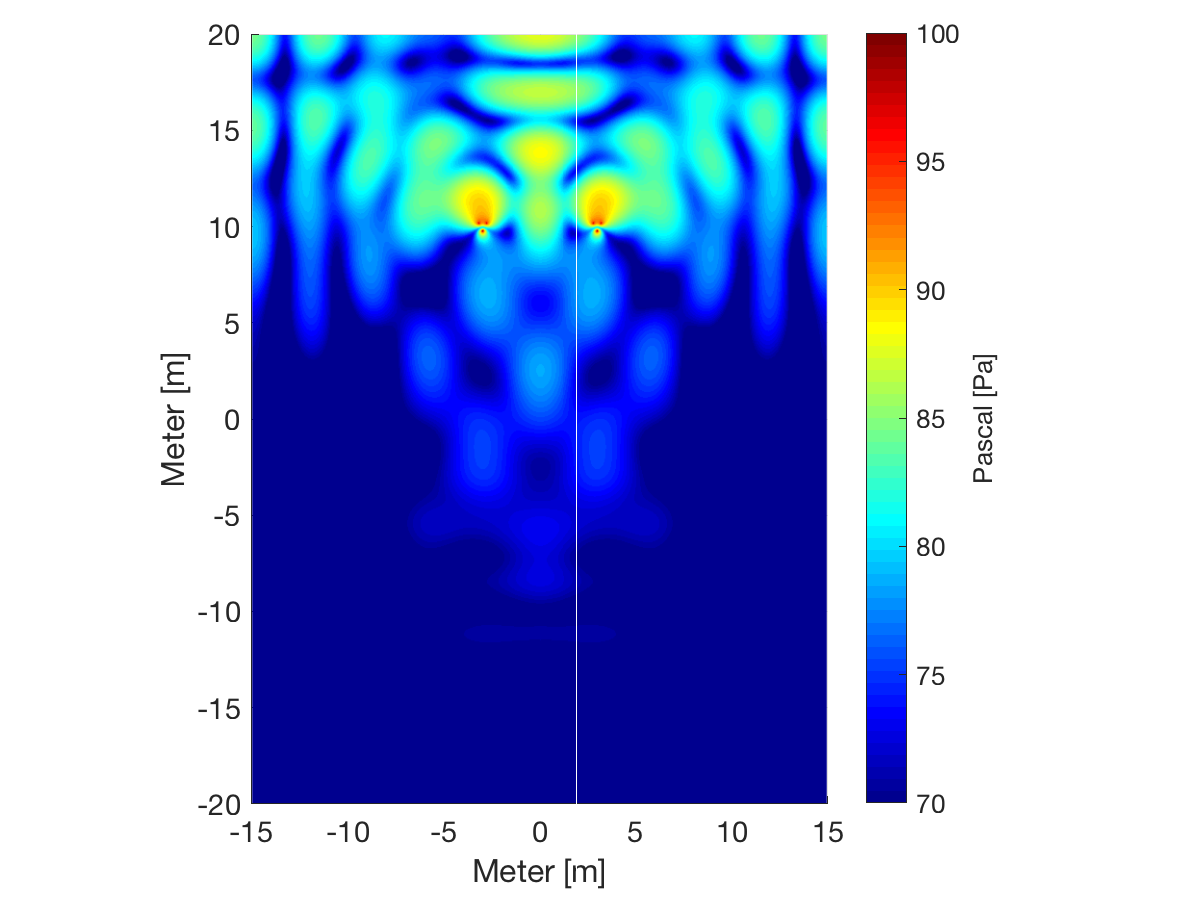
\includegraphics[width=0.95\textwidth]{60_hz_monitor_beam.eps}
\subcaption{Indoor simulation of  \SI{60}{\hertz} with beamforming}
\label{fig:Indoor_monitor_60_on}
\end{subfigure}
\begin{subfigure}[c]{0.5\textwidth}
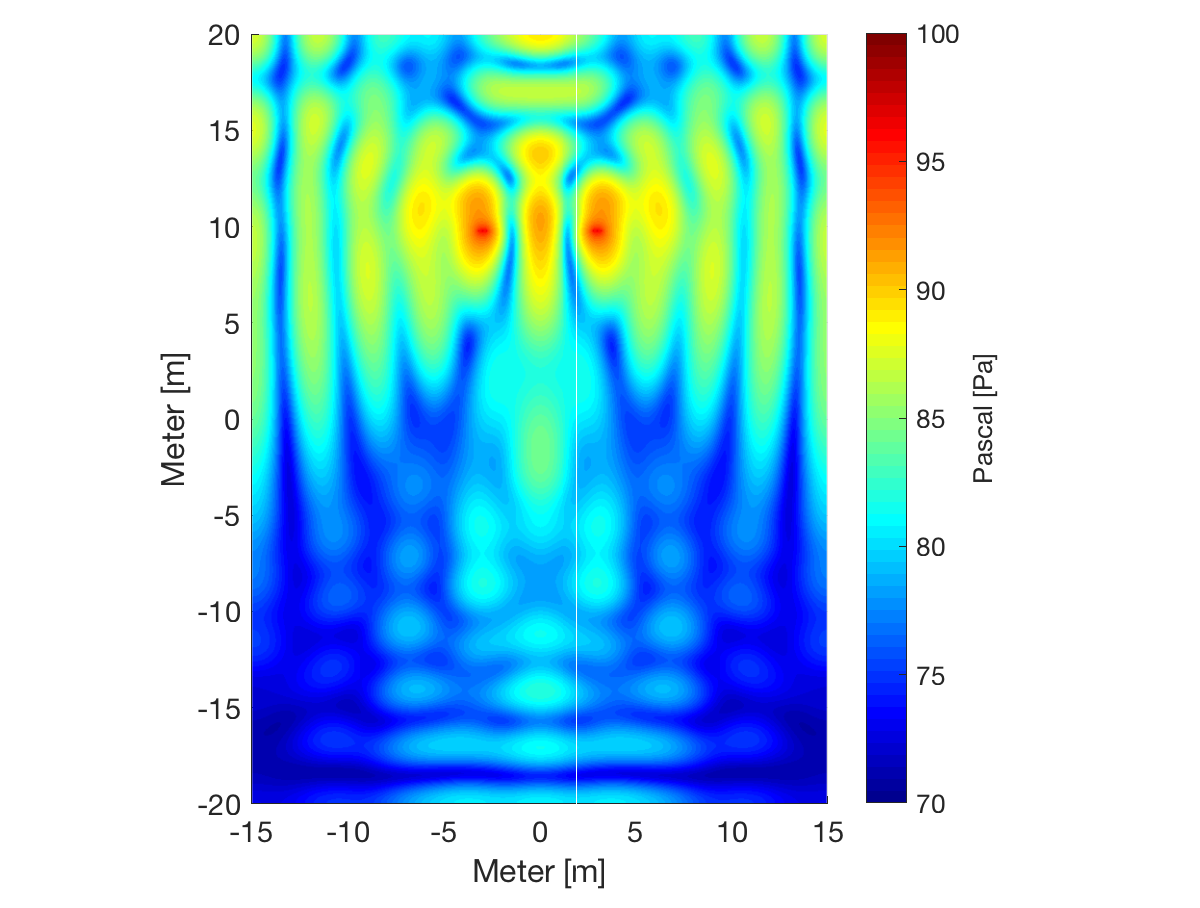
\includegraphics[width=0.95\textwidth]{60_hz_monitor_without_beam.eps}
\subcaption{Indoor simulation of  \SI{60}{\hertz} without beamforming}
\label{fig:Indoor_monitor_60_off}
\end{subfigure}\\
\hspace{0.1\textheight}
\begin{subfigure}[c]{0.5\textwidth}
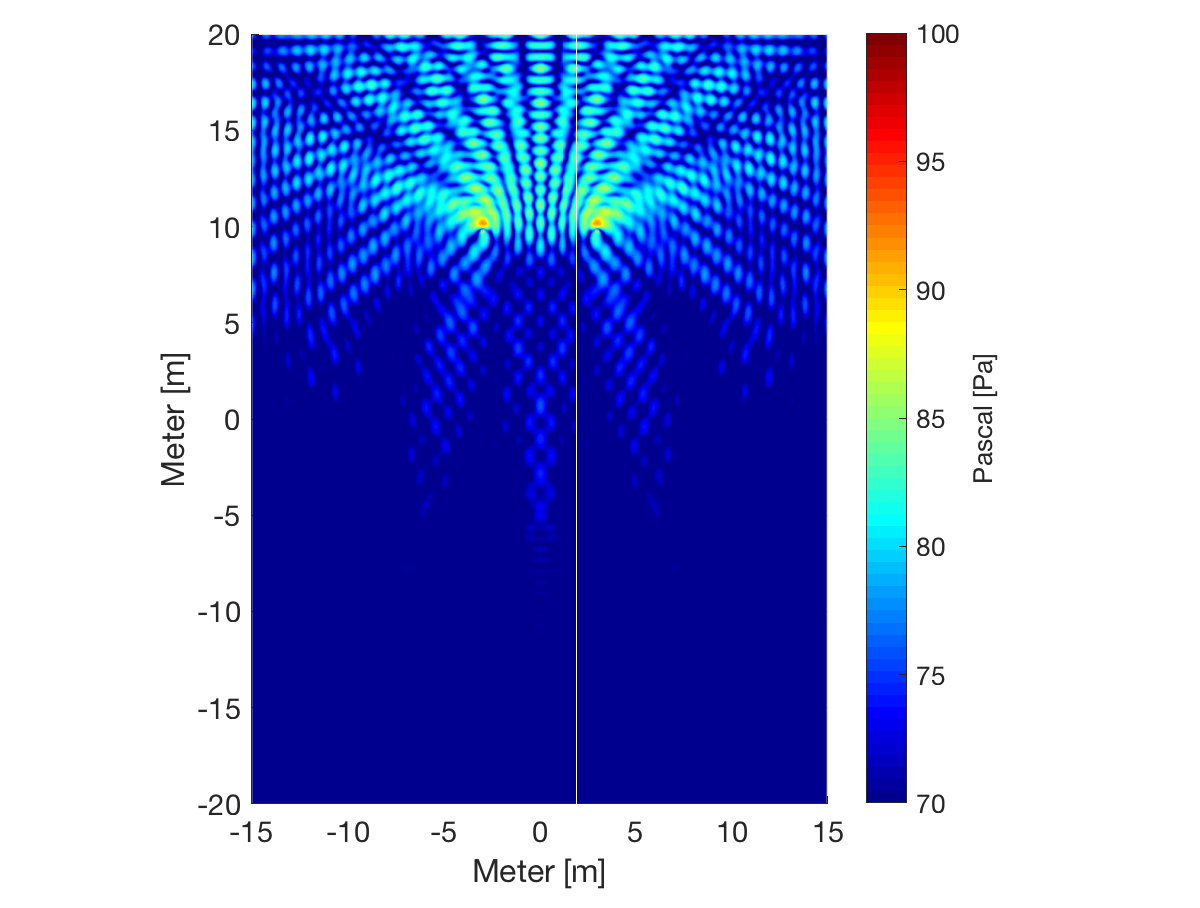
\includegraphics[width=0.95\textwidth]{300_hz_monitor_beam.eps}
\subcaption{Indoor simulation of  \SI{100}{\hertz} with beamforming}
\label{fig:Indoor_monitor_300_on}
\end{subfigure}
\begin{subfigure}[c]{0.5\textwidth}
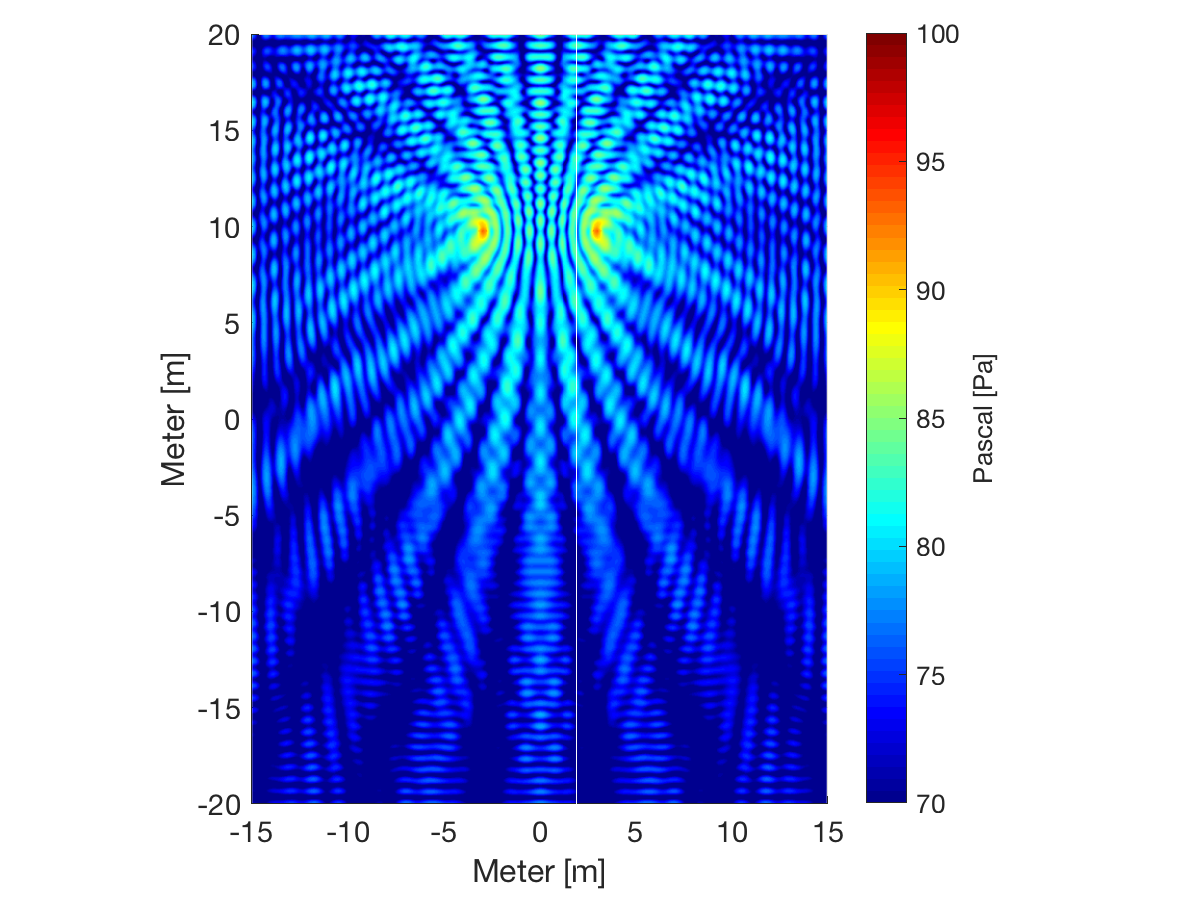
\includegraphics[width=0.95\textwidth]{300_hz_monitor_without_beam.eps}
\subcaption{Indoor simulation of  \SI{100}{\hertz} with beamforming}
\label{fig:Indoor_monitor_300_off}
\end{subfigure}
\caption{The figure shows a 2 dimension \gls{fdtd} simulation in a monitor application}
		\label{fig:Indoor_monitor_60_300}
\end{figure}

In \autoref{fig:Indoor_monitor_60_300} it can be seen that the two monitor playing cardioid mostly have an effect on the audience and do not change much on stage. On change to the monitoring system might be that those two monitors was changed with only one beamforming monitor, but feeded with to signals and different beamforming. So one signal is playing to the left of the monitor, there the other signal was playing to the right. This concept have not been tested but it might be one possibility for change of the beamforming system.


\section{Conclusion of discussion}
